\section{Kinematics}
\subsection{Vector notation}
There are two ways of expressing vectors:
\begin{subequations}
\begin{align}
    \mathbf{r}^i &= \begin{bmatrix} a \\ b \\ c \end{bmatrix} \\
    \vec{r}_{a/b} &= a\vec{i}_i + b\vec{j}_i + c\vec{k}_i
\end{align}
\end{subequations}
Where $i$ is the frame of reference, and subscript $a/b$ denotes from point b to point a. If the vectors are velocities, subscript $a/b$ denotes the velocity of point a relative to point b.
It is important to be consistent in the notation. Never do arithmetic operations on vectors expressed in different frames. This means: \newline
\begin{subequations}
\begin{align}
    \bcancel{\cancel{\vec{r}^i}}\\
    \bcancel{\cancel{\mathbf{v}^i+\mathbf{u}^a}}\\
    \bcancel{\cancel{\mathbf{v}^i \times \mathbf{u}^a}}
\end{align}
\end{subequations}

\subsection{Skew matrix notation}
If you have $\mathbf{u} = \begin{bmatrix}u_1 & u_2 & u_3\end{bmatrix}^\top$ and $\mathbf{v} = \begin{bmatrix}v_1 & v_2 & v_3\end{bmatrix}^\top$:
\begin{subequations}
    \begin{align}
    \mathbf{u}^\times = \begin{bmatrix}
                    0 & -u_3 & u_2 \\
                    u_3 & 0 & -u_1 \\
                    -u_2 & u_1 & 0
                  \end{bmatrix} \\
    \mathbf{u}^\times \mathbf{v} = \mathbf{u} \times \mathbf{v} \\
    \mathbf{u}^\times \mathbf{u} = 0 \\
    \left(\mathbf{u}^\times\right)^\times = -\mathbf{u}^\times \\
    \det{(\mathbf{u}^\times)} = 0  
    \end{align}
\end{subequations}
The cross product of two vectors can be calculated by finding the determinant of this matrix:
\begin{equation}
    \mathbf{u} \times \mathbf{v} = \det{\begin{bmatrix}
                    \vec{i} & \vec{j} & \vec{k} \\
                    u_1 & u_2 & u_3 \\
                    v_1 & v_2 & v_3
                  \end{bmatrix}}
\end{equation}

\subsection{Rotation matrices}
The rotation matrices are defined on each axis as:
\begin{subequations}
    \begin{align}
    \mathbf{R}_x(\theta) &= \begin{bmatrix} 1 & 0 & 0 \\ 0 & \cos(\theta) & -\sin(\theta) \\ 0 & \sin(\theta) & \cos(\theta) \end{bmatrix} \\
    \mathbf{R}_y(\phi) &= \begin{bmatrix} \cos(\phi) & 0 & \sin(\phi) \\ 0 & 1 & 0 \\ -\sin(\phi) & 0 & \cos(\phi) \end{bmatrix} \\
    \mathbf{R}_z(\psi) &= \begin{bmatrix} \cos(\psi) & -\sin(\psi) & 0 \\ \sin(\psi) & \cos(\psi) & 0 \\ 0 & 0 & 1 \end{bmatrix}
    \end{align}
\end{subequations}
Now lets say frame $a$ relative to frame $i$ is rotated by $\theta$ about the $x$-axis, $\phi$ about the $y$-axis, and $\psi$ about the $z$-axis. The rotation matrix from frame $a$ to frame $i$ is then:
\begin{equation}
    \mathbf{R}_i^a = \mathbf{R}_z(\psi)\mathbf{R}_y(\phi)\mathbf{R}_x(\theta)
\end{equation}
Which means that $\mathbf{R}_i^a$ is called the \textit{rotation matrix} from frame $a$ to frame $i$. \newline
\begin{figure}[H]
    \centering
    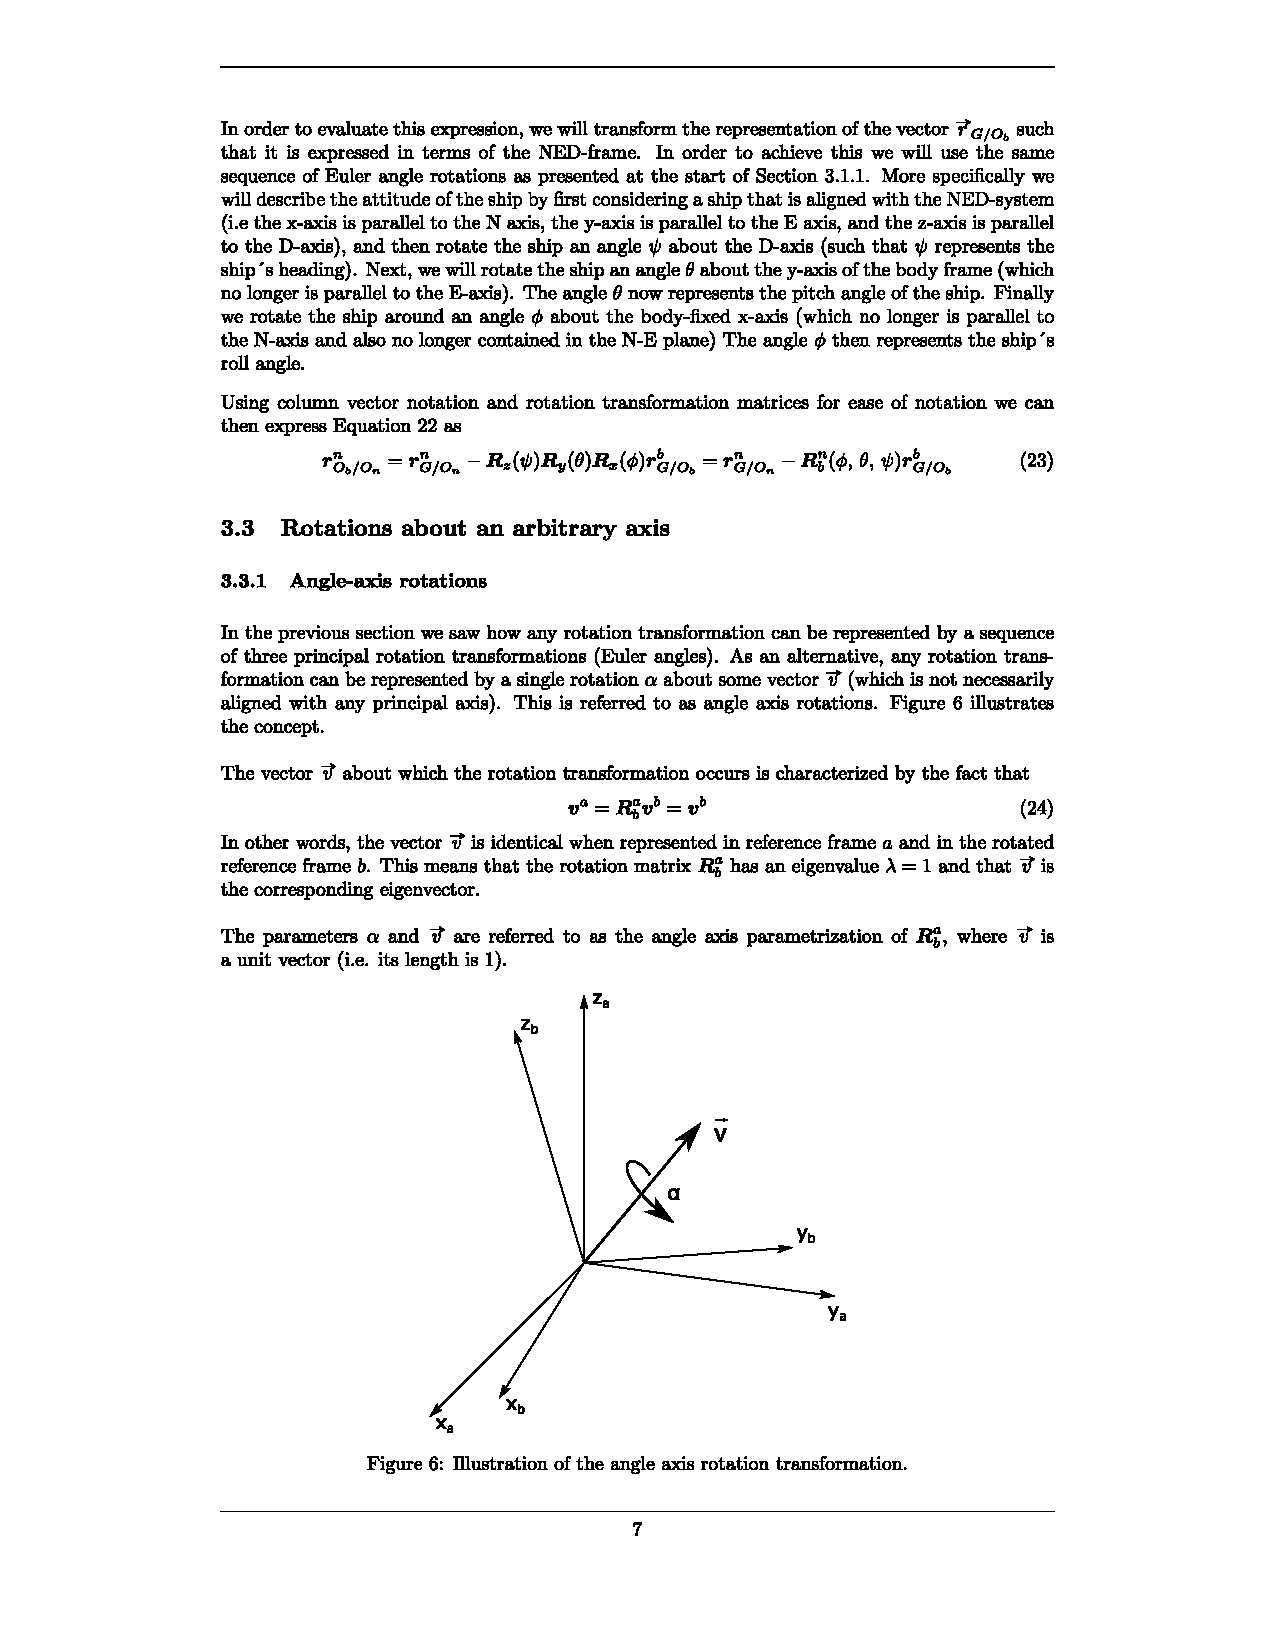
\includegraphics[scale=1, trim={7cm 3.5cm 7cm 16.5cm}, clip]{figures/arbitrary_axis_rotation.pdf}
    \caption{Rotation about arbitrary axis}
    \label{fig:arbitrary_axis_rotation}
\end{figure}
Now, if we have a rotation about an arbitrary axis $\mathbf{v}$, we can use the equation:
\begin{equation}
    \mathbf{R}_{\alpha,\vec{v}} = \cos(\alpha)\mathbf{I} + \mathbf{v}^\times\sin(\alpha) + \mathbf{vv}^\top(1-\cos(\alpha)) = \mathbf{R}_b^a(\alpha)
\end{equation}
\subsubsection{Properties of rotation matrices}
A couple of maybe interesting properties of rotation matrices:
\begin{subequations}
    \begin{align}
        \mathbf{v}^b=\mathbf{R}_a^b\mathbf{v}^a \\
        \mathbf{v}^a=\mathbf{R}_b^a\mathbf{v}^b \\
        \mathbf{R}_a^b\mathbf{R}_b^a = \mathbf{I} \\
        \mathbf{R}_a^b = \left(\mathbf{R}_b^a\right)^{-1} = \left(\mathbf{R}_b^a\right)^\top \\
        \dot{\mathbf{R}}_b^a = \left(\mathbf{\omega}_{ab}^a\right)^\times\mathbf{R}_b^a = \mathbf{R}_b^a\left(\mathbf{\omega}_{ab}^b\right)^\times \\
        \left(\vec{\omega}_{ab}^a\right)^\times = \dot{\mathbf{R}}_b^a\left(\mathbf{R}_b^a\right)^\top \\
        \vec{\omega}_{ad} = \vec{\omega}_{ab} + \vec{\omega}_{bc} + \vec{\omega}_{cd}
    \end{align}
\end{subequations}
Where the vector $\vec{\omega}_{ab}^a$ is the angular velocity vector from frame \textit{b} relative to frame \textit{b} with respect to frame \textit{a}.
\subsection{Other stuff that might be usefull}
\textbf{Linear momentum} does not depend upn its point of reference:
\begin{subequations}
    \begin{align}
        \vec{p} = m\vec{v} \\
        \dot{\vec{p}} = m\vec{a} = \vec{F}
    \end{align}
\end{subequations}
\textbf{Angular momentum} of point \textit{p} with respect t origin \textit{o}, where $\vec{r}_{p/o}$ is the position of \textit{p} and $\vec{p}$ is the linear momentum. (Angular momentum depends upon its point of reference):
\begin{subequations}
    \begin{align}
        \vec{h}_{p/o} = \vec{r}_{p/o} \times \vec{p} \\
        \dot{\vec{h}}_{p/o} = \vec{r}_{p/o} \times \dot{\vec{p}} = \vec{T}
    \end{align}
\end{subequations}